\documentclass{ctexart}
 
\usepackage{pgf}
\usepackage{tikz}
\usetikzlibrary{arrows, decorations.pathmorphing, backgrounds, positioning, fit, petri, automata}

\usetikzlibrary{shapes.geometric,shadows,shapes.symbols}
\definecolor{yellow1}{rgb}{1,0.8,0.2} 
 
%opening
\begin{document}
    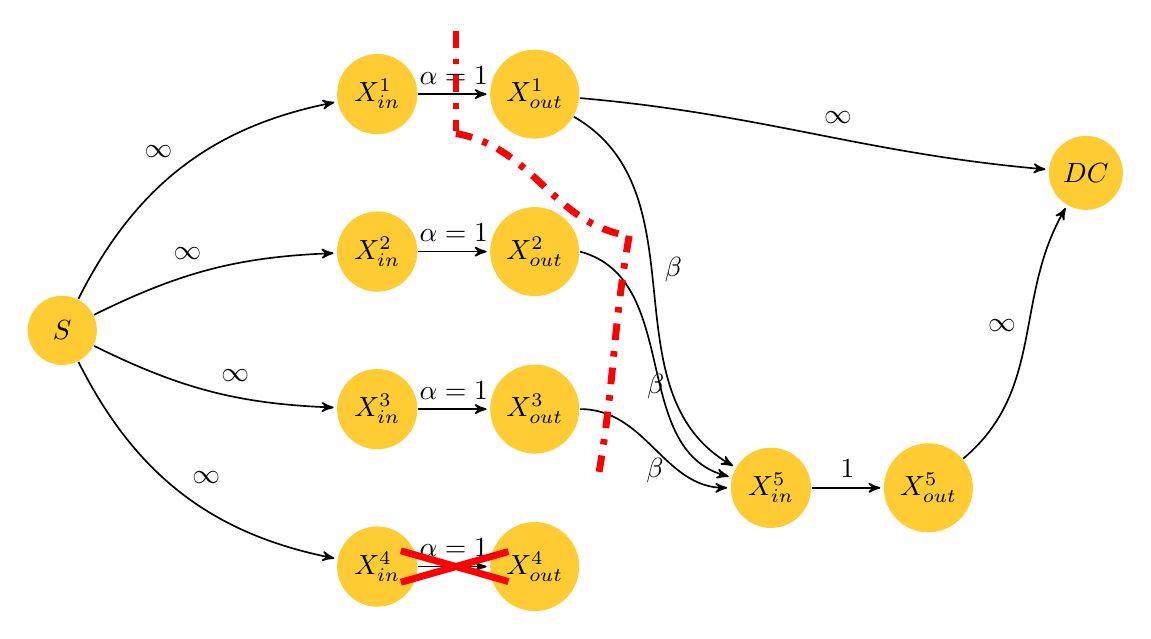
\begin{tikzpicture}[->,>=stealth',shorten >=1pt,auto,node distance=2.8cm,
                    semithick]
        \tikzstyle{every state}=[fill=yellow1,draw=none,text=black]
 
        \node[state]         (S) at (-6, 0)              {$S$};
        \node[state]         (xin1) at (-2, 3)           {$X^1_{in}$};
        \node[state]         (xin2) at (-2, 1)        {$X^2_{in}$};
        \node[state]         (xin3) at (-2, -1)       {$X^3_{in}$};
        \node[state]         (xin4) at (-2, -3)           {$X^4_{in}$};
        \node[state]         (xout1) at (0, 3)          {$X^1_{out}$};
        \node[state]         (xout2) at (0, 1)        {$X^2_{out}$};
        \node[state]         (xout3) at (0, -1)   {$X^3_{out}$};
        \node[state]         (xout4) at (0, -3)           {$X^4_{out}$};
        \node[state]         (xin5)  at (3, -2)   {$X^5_{in}$};
        \node[state]         (xout5) at (5, -2)   {$X^5_{out}$};
        \node[state]         (DC) at (7, 2)           {$DC$};
 
        \path (S) edge[bend left=26]              node {$\infty$} (xin1)
            edge[bend left=12]              node {$\infty$} (xin2)
            edge[bend right=12]             node {$\infty$} (xin3)
            edge[bend right=26]             node {$\infty$} (xin4)
            (xin1) edge  node {$\alpha=1$} (xout1)
            (xin2) edge  node {$\alpha=1$} (xout2)
            (xin3) edge  node {$\alpha=1$} (xout3)
            (xin4) edge  node {$\alpha=1$} (xout4)
            (xin5) edge  node {$1$} (xout5);
        \draw[->] (xout1) to[out=-30,in=150] node {$\beta$} (xin5);
        \draw[->] (xout2.east) to[out=-15,in=165] node [below] {$\beta$} (xin5);
        \draw[->] (xout3.east) to[out=0,in=180] node [below] {$\beta$} (xin5.west);
        \draw[->] (xout1) to[out=-5,in=175] node {$\infty$} (DC);
        \draw[->] (xout5) to[out=40, in=-120] node {$\infty$} (DC);

        \draw[line width=2.5pt,red,-] (-1.7,-2.8)--(-0.3,-3.2);
        \draw[line width=2.5pt,red,-] (-1.7,-3.2)--(-0.3,-2.8);
 
        \draw[line width=2.5pt,red,dash pattern=on 6pt off 4pt on 2pt off 4pt,-] (-1,3.8)--(-1,2.5);
        \draw[line width=2.5pt,red,dash pattern=on 6pt off 4pt on 2pt off 4pt,-] (-1,2.5) to[out=-10,in=170] (1.2,1.2);
        \draw[line width=2.5pt,red,dash pattern=on 6pt off 4pt on 2pt off 4pt,-] (1.2,1.2) to[out=-100,in=80] (0.8,-1.9);
    \end{tikzpicture}

    \tikz{
        \node  (A) at (0,0) {全响应$r(t)$=};
        \node  (B) at (2.7,0) {零输入响应$r_{zi}(t)$+};
        \node  (C) at (5.7,0) {零状态响应$r_{zs}(t)$};
        \node[align=left,anchor=north]  (D) at (2.7,-1.5) {解齐次方程\\代入初始条件\\确定系数};
        \draw[ultra thick][-latex'] (B) to (D);
        \node[align=left,anchor=north]  (E) at (5.7,-1.5) {卷积积分\\$e(t)\ast h(t)$};
        \draw[ultra thick][-latex'] (C) to (E);
    }


    \tikz \draw (0,0) node[anchor=south east] {first node} rectangle (1,1) node[anchor=west] {second node};

    \tikz{
        \fill[fill=yellow!80!black]
        (0,0) node {first node}
        -- (1,1) node[draw, behind path] {second node}
        -- (0,2) node[fill=red!20,draw,double,rounded corners] {third node};
    }

    \tikz{
        \fill[fill=yellow!80!black]
        (0,0) node {first node}
        -- (1,1) node[ellipse,draw, behind path] {second node}
        -- (0,2) node[circle,fill=red!20] {third node};
    }
    

    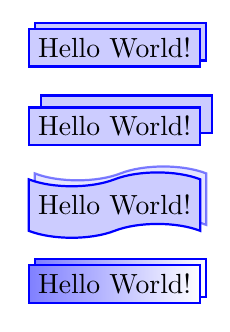
\begin{tikzpicture}
        \node [copy shadow,fill=blue!20,draw=blue,thick] {Hello World!};
        \node at (0,-1) [copy shadow={shadow xshift=1ex,shadow yshift=1ex},
            fill=blue!20,draw=blue,thick] {Hello World!};
        \node at (0,-2) [copy shadow={opacity=.5},tape,
            fill=blue!20,draw=blue,thick] {Hello World!};
        % We have to repeat the left color since shadings are not
        % automatically applied to shadows
        \node at (0,-3) [copy shadow={left color=blue!50},
            left color=blue!50,draw=blue,thick] {Hello World!};
    \end{tikzpicture}

    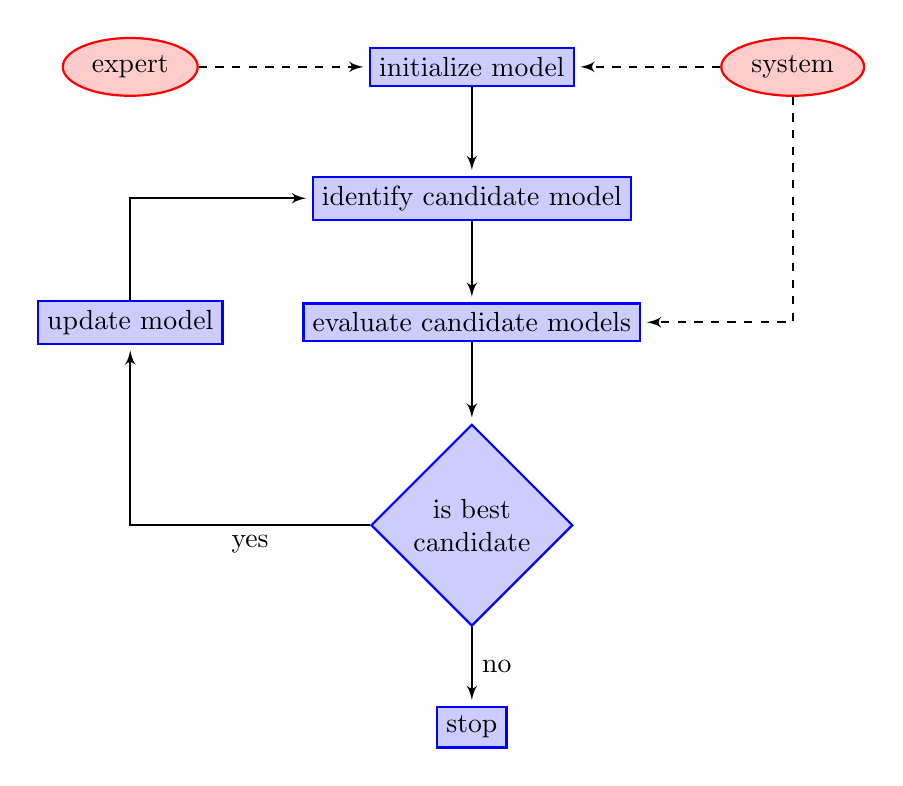
\begin{tikzpicture}
        [auto,
        decision/.style={diamond, draw=blue, thick, fill=blue!20,
        text width=5em,
        align=flush center,
        inner sep=1pt},
        block/.style ={rectangle, draw=blue, thick, fill=blue!20,
        %text width=5em,align=center, rounded corners,
        %minimum height=4em
        },
        line/.style ={draw, thick,-latex',shorten >=2pt},
        cloud/.style ={draw=red, thick, ellipse,fill=red!20,
        minimum height=2em}]
        \matrix [column sep=10mm,row sep=10mm]
            {
                % row 1
                \node [cloud] (expert) {expert}; &
                \node [block] (init) {initialize model}; &
                \node [cloud] (system) {system}; \\
                % row 2
                & \node [block] (identify) {identify candidate model}; & \\
                % row 3
                \node [block] (update) {update model}; &
                \node [block] (evaluate) {evaluate candidate models}; & \\
                % row 4
                & \node [decision] (decide) {is best candidate}; & \\
                % row 5
                & \node [block] (stop) {stop}; & \\
        };
        \begin{scope}[every path/.style=line]
            \path (init) -- (identify);
            \path (identify) -- (evaluate);
            \path (evaluate) -- (decide);
            \path (update) |- (identify);
            \path (decide) -| node [near start] {yes} (update);
            \path (decide) -- node [midway] {no} (stop);
            \path [dashed] (expert) -- (init);
            \path [dashed] (system) -- (init);
            \path [dashed] (system) |- (evaluate);
        \end{scope}
    \end{tikzpicture}

    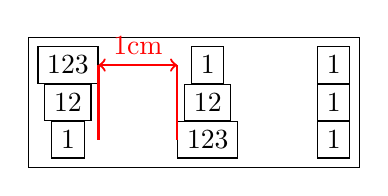
\begin{tikzpicture}
        \matrix [draw,column sep=1cm,nodes=draw]
        {
            \node(a) {123}; & \node (b) {1}; & \node {1}; \\
            \node {12}; & \node {12}; & \node {1}; \\
            \node(c) {1}; & \node (d) {123}; & \node {1}; \\
        };
        \draw [red,thick] (a.east) -- (a.east |- c)
        (d.west) -- (d.west |- b);
        \draw [<->,red,thick] (a.east) -- (d.west |- b)
        node [above,midway] {1cm};
    \end{tikzpicture}
    
\end{document}